\section{Dataset and Experimental Protocol}
\subsection{V2X-Sim Release and Evaluation Units}
V2X-Sim provides simulated multi-agent observations and annotations for
collaborative perception~\cite{li2022v2xsim}. The source recordings include
vehicle and roadside sensors, but the experiments here exclude roadside-unit
inputs. Cameras provide visual context; they are not inputs to this LiDAR
detector. The official scene partitions and the recorded vehicle-only counts
are summarized in Table~\ref{tab:dataset}.

\begin{table}[htbp]
\centering
\caption{V2X-Sim 2.0 scene partitions used by the released detection protocol.}
\label{tab:dataset}
\begin{ReportTable}{Lrrrr}
\ReportTableHead
\ReportTH{Partition} & \ReportTH{Scenes} & \ReportTH{Frames} & \ReportTH{Vehicle inputs/frame} & \ReportTH{Vehicle scans} \\
Train & 80 & 8,000 & 2--5 & 29,200 \\
Validation & 10 & 1,000 & 3--5 & 4,000 \\
Test & 10 & 1,000 & 3--5 & 4,000 \\
\rowcolor{ReportTableSummary}
\textbf{Total} & \textbf{100} & \textbf{10,000} & --- & \textbf{37,200} \\
\end{ReportTable}
\end{table}

One synchronized frame contains observations from several active vehicles.
One \emph{vehicle view} is the output of one active vehicle at one frame.
The full test split contains 300 frames with three vehicles, 400 with four,
and 300 with five, giving 4,000 active views. Matching is performed within
each view; predictions are then pooled for AP. An object observed by two
vehicles contributes a reference box in each vehicle's evaluation view.
The 50,047 reference boxes in the benchmark therefore count view-specific
references, not unique physical cars across the recordings. The views are
also correlated observations, not 4,000 independent synchronized frames.

The original DiscoNet paper evaluates V2X-Sim 1.0, whereas this study uses
the prepared 2.0 detection release. CoPerception's documentation identifies
2.0 as its supported release~\cite{coperceptiondata}. The results are an
evaluation of that released implementation and checkpoint, not an exact
reproduction of the paper's 1.0 benchmark numbers.

\subsection{Model, Hardware, and Software}
All three experiments use the unchanged epoch-100 DiscoNet student in
float32 precision on one NVIDIA GeForce RTX 5060 Ti with approximately 16 GB
of GPU memory. The recorded setup has an AMD Ryzen 7 5700X CPU with eight
cores and sixteen threads, approximately 16 GB of system RAM, and Omarchy
Linux. The experiment environment records Python 3.14.8, PyTorch
2.9.1+cu128, and CUDA runtime 12.8.
The following results use this recorded configuration.

The checkpoint contains 15,843,505 parameters and is loaded with a strict
state-dictionary check. The inference implementation is pinned to source
commit \texttt{dd8fbb660300}. Its checkpoint hash and run identities are
stored with the evaluation records in the project repository.
No training, checkpoint selection, or parameter update is performed in the
reported evaluations.

\subsection{Detection Metrics and Postprocessing}
\label{sec:metrics}
Intersection over Union measures overlap between a prediction $B_p$ and
its reference box $B_g$:
\[
  \operatorname{IoU}(B_p,B_g)=
    \frac{|B_p\cap B_g|}{|B_p\cup B_g|}.
\]
AP is reported at matching thresholds of 0.5 and 0.7. The larger threshold
requires more accurate localization.

\begin{figure}[htbp]
\centering
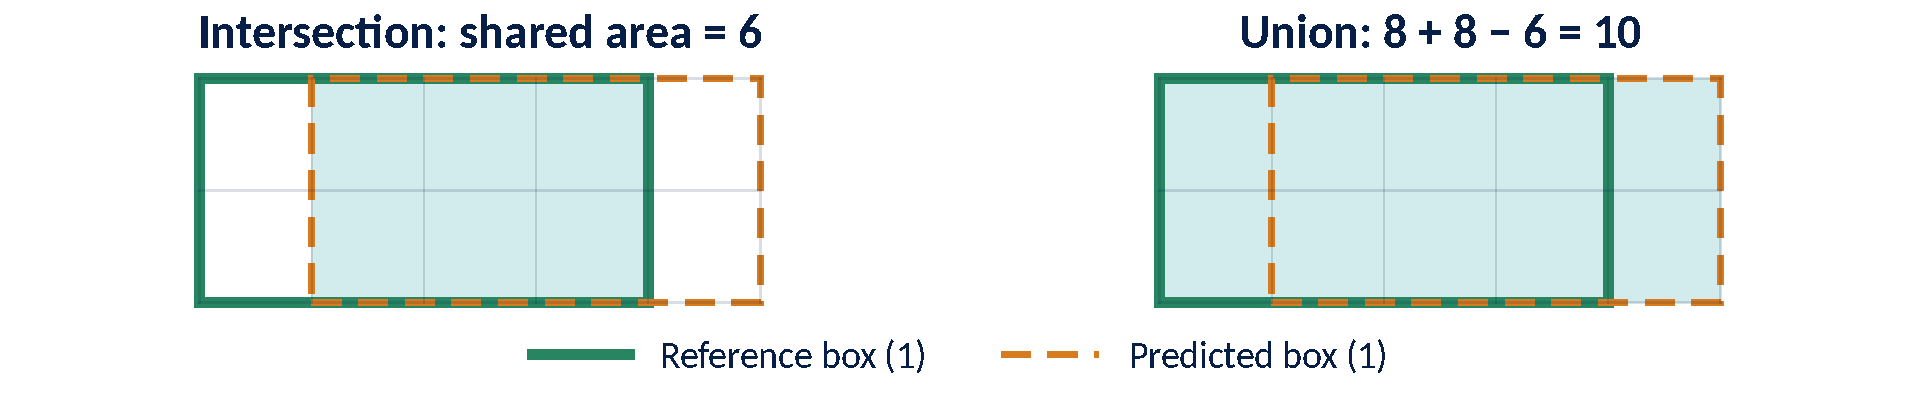
\includegraphics[width=\linewidth]{metrics/iou-overlap-v1.pdf}
\caption[Worked intersection and union areas]{Project IoU example. Both
rectangles have area eight, their intersection has area six, and their
union has area ten. The geometry is illustrative.}
\label{fig:iou-overlap}
\end{figure}

Figure~\ref{fig:iou-overlap} gives a concrete calculation:
\[
 \operatorname{IoU}=\frac{6}{8+8-6}=\frac{6}{10}=0.60.
\]
That prediction qualifies at a 0.5 matching threshold but fails at 0.7.
Figure~\ref{fig:iou-thresholds} extends the comparison to three overlaps.
The reference box is held fixed while the displacement of the prediction
changes. A stricter matching threshold asks for closer agreement with the
reference geometry.

\begin{figure}[htbp]
\centering
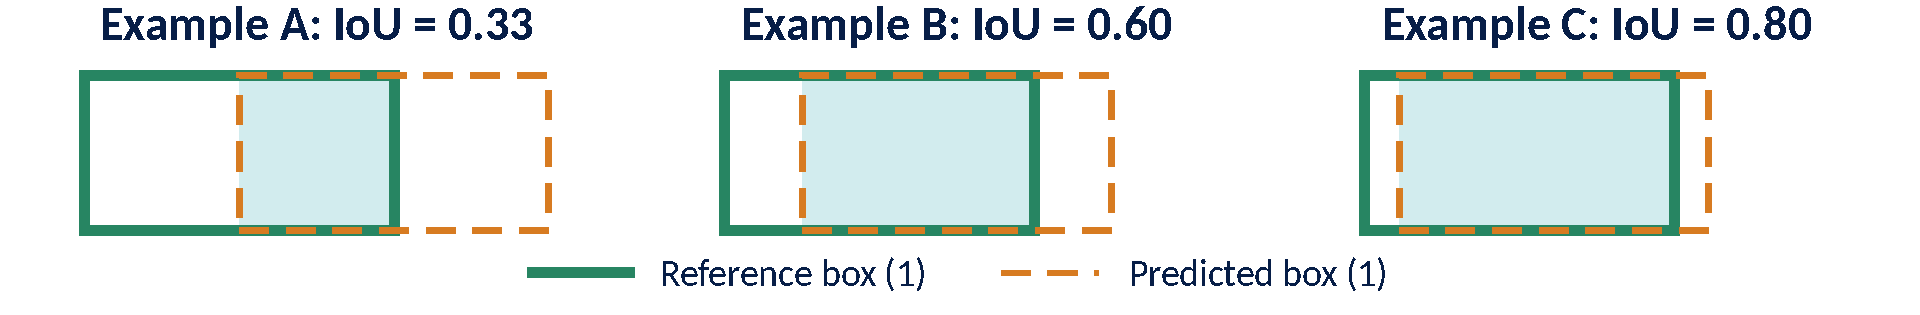
\includegraphics[width=\linewidth]{metrics/iou-thresholds-v1.pdf}
\caption[Three overlaps under the two matching thresholds]{Project geometry
examples with IoU approximately 0.33, 0.60, and 0.80. Only the last two
qualify at 0.5; only the last qualifies at 0.7.}
\label{fig:iou-thresholds}
\end{figure}

\FloatBarrier
\subsection{Confidence Scores and Retained Predictions}
The retained car score is obtained by a softmax of background and car logits:
\[
 p_{\mathrm{car}}=
 \frac{e^{z_{\mathrm{car}}}}{e^{z_{\mathrm{background}}}+e^{z_{\mathrm{car}}}}.
\]
The recorded evaluation keeps confidence strictly greater than 0.7 and uses
rotated nonmaximum suppression (NMS) with IoU 0.01. Confidence filtering
removes low-scoring candidates; NMS suppresses overlapping candidate
predictions. These operations precede matching to reference boxes.

\begin{table}[htbp]
\centering
\caption{The project's illustrative logits-to-confidence example.}
\label{tab:confidence-example}
\begin{ReportTable}{lRRRc}
\ReportTableHead
\ReportTH{Box} & \ReportTH{Background logit} & \ReportTH{Car logit} & \ReportTH{Car score} & \ReportTH{Score $>0.7$} \\
A & 1.0 & 3.0 & 0.881 & Keep \\
B & 2.0 & 1.0 & 0.269 & Discard \\
C & 1.0 & 4.0 & 0.953 & Keep \\
\end{ReportTable}
\end{table}

For Box A in Table~\ref{tab:confidence-example}, the conversion is
$e^3/(e^1+e^3)\approx0.881$. Box C ranks above A because its car score is
higher. Box B is removed by the confidence filter. These logits are the
worked example from the project slides, rather than outputs selected from
the benchmark.

Three thresholds have different jobs. The confidence threshold acts on a
class score. The NMS IoU threshold compares predictions with other
predictions. The evaluation IoU thresholds compare retained predictions
with reference boxes. Thus the score threshold of 0.7 and matching
threshold of 0.7 do not describe the same test.

\subsection{Precision, Recall, and Average Precision}
Predictions are ranked by their
car-class confidence, matched one-to-one within their vehicle view, and
classified as true positives (TP) or false positives (FP). Duplicate and
unmatched predictions are false positives. Precision and recall are
\[
  P=\frac{\mathrm{TP}}{\mathrm{TP}+\mathrm{FP}},\qquad
  R=\frac{\mathrm{TP}}{N_{\mathrm{reference}}}.
\]
AP integrates the interpolated precision envelope as recall increases.
It combines detection coverage and false-positive control; prediction count
alone is not AP.

Table~\ref{tab:ap-example} and Figure~\ref{fig:ap-example} reproduce the
project's four-prediction example with three reference cars. The first
prediction matches a reference. The second is a false positive, so recall
stays at $1/3$ and precision falls to $1/2$. The last two predictions match
the remaining references. Each reference can be credited only once.

\begin{table}[htbp]
\centering
\caption{Worked AP example with three reference cars and IoU matching at 0.5.}
\label{tab:ap-example}
\begin{ReportTable}{rrlRRR}
\ReportTableHead
\ReportTH{Rank} & \ReportTH{Score} & \ReportTH{Result} & \ReportTH{Cumulative TP / FP} & \ReportTH{Precision} & \ReportTH{Recall} \\
1 & 0.99 & TP & 1 / 0 & 100.0\% & 33.3\% \\
2 & 0.96 & FP & 1 / 1 & 50.0\% & 33.3\% \\
3 & 0.92 & TP & 2 / 1 & 66.7\% & 66.7\% \\
4 & 0.83 & TP & 3 / 1 & 75.0\% & 100.0\% \\
\end{ReportTable}
\end{table}

\begin{figure}[htbp]
\centering
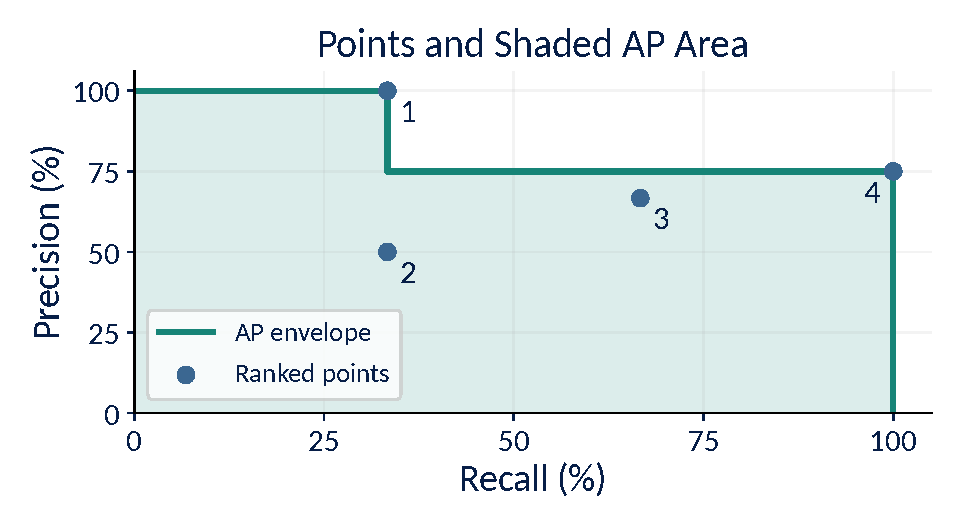
\includegraphics[width=0.76\linewidth]{metrics/ap-example-curve-v1.pdf}
\caption[A worked precision--recall curve and its envelope]{The project's
illustrative AP curve for Table~\ref{tab:ap-example}. The precision envelope
uses the best precision available at or beyond each recall level.}
\label{fig:ap-example}
\end{figure}

The interpolated envelope has precision one over the first third of recall
and $0.75$ over the remaining two thirds. Its area is
\[
 \operatorname{AP}=\tfrac13\times1+
                   \tfrac13\times0.75+
                   \tfrac13\times0.75
                 =\tfrac56\approx83.3\%.
\]
The false positive is present in the ranking even though every reference
eventually receives a match. Conversely, missed or filtered-out references
limit the maximum recall. The full-test curves in Section~\ref{sec:benchmark}
apply this evaluation to the recorded population rather than this small
teaching example.

\FloatBarrier

\subsection{Three Evidence Sets}
\label{sec:evidence-sets}
The full-test experiment compares sharing off and on over all 1,000 test
frames. The runtime-only experiment uses 30 fixed frames and measures
$n=1,\ldots,20$ slots without AP. The Original/Tree comparison uses 30 fixed
ego-1 views and measures both runtime and AP for $n=1,\ldots,15$.
The latter two use ten frames each from raw scenes \texttt{scene\_9},
\texttt{scene\_97}, and \texttt{scene\_98}. Their separately recorded timings
must not be substituted for one another. AP from the ego-only ablation is
also not directly comparable to AP pooled over all full-test vehicle views.

\begin{table}[htbp]
\centering
\caption{The three experiment populations and the questions they answer.}
\label{tab:evidence-sets}
\begin{ReportTable}{P{0.18\linewidth}P{0.28\linewidth}L}
\ReportTableHead
\ReportTH{Evidence set} & \ReportTH{Population} & \ReportTH{Reported outputs} \\
Full test & 1,000 synchronized frames; 4,000 active vehicle views &
  AP and fixed-checkpoint loss with sharing off/on \\
Runtime sweep & 30 recorded frames; 1--20 input slots &
  Full-group forward median and P95; no AP \\
Original/Tree & 30 ego-1 views; 427 reference cars; 1--15 slots &
  Matched forward medians and ego-view AP for both methods \\
\end{ReportTable}
\end{table}

Table~\ref{tab:evidence-sets} gives the denominator for each result before
the numerical comparisons. A synchronized frame, a vehicle view, an input
slot, and a timed forward are different units. Repeating a forward yields
another runtime sample, while repeating a scan in another slot changes the
computational workload. Neither operation creates a new independent
reference scene.
